\documentclass[]{article}
\usepackage{lmodern}
\usepackage{amssymb,amsmath}
\usepackage{ifxetex,ifluatex}
\usepackage{fixltx2e} % provides \textsubscript
\ifnum 0\ifxetex 1\fi\ifluatex 1\fi=0 % if pdftex
  \usepackage[T1]{fontenc}
  \usepackage[utf8]{inputenc}
\else % if luatex or xelatex
  \ifxetex
    \usepackage{mathspec}
  \else
    \usepackage{fontspec}
  \fi
  \defaultfontfeatures{Ligatures=TeX,Scale=MatchLowercase}
\fi
% use upquote if available, for straight quotes in verbatim environments
\IfFileExists{upquote.sty}{\usepackage{upquote}}{}
% use microtype if available
\IfFileExists{microtype.sty}{%
\usepackage{microtype}
\UseMicrotypeSet[protrusion]{basicmath} % disable protrusion for tt fonts
}{}
\usepackage[margin=1in]{geometry}
\usepackage{hyperref}
\hypersetup{unicode=true,
            pdftitle={Homework 02},
            pdfauthor={Jiahao Xu},
            pdfborder={0 0 0},
            breaklinks=true}
\urlstyle{same}  % don't use monospace font for urls
\usepackage{color}
\usepackage{fancyvrb}
\newcommand{\VerbBar}{|}
\newcommand{\VERB}{\Verb[commandchars=\\\{\}]}
\DefineVerbatimEnvironment{Highlighting}{Verbatim}{commandchars=\\\{\}}
% Add ',fontsize=\small' for more characters per line
\usepackage{framed}
\definecolor{shadecolor}{RGB}{248,248,248}
\newenvironment{Shaded}{\begin{snugshade}}{\end{snugshade}}
\newcommand{\KeywordTok}[1]{\textcolor[rgb]{0.13,0.29,0.53}{\textbf{#1}}}
\newcommand{\DataTypeTok}[1]{\textcolor[rgb]{0.13,0.29,0.53}{#1}}
\newcommand{\DecValTok}[1]{\textcolor[rgb]{0.00,0.00,0.81}{#1}}
\newcommand{\BaseNTok}[1]{\textcolor[rgb]{0.00,0.00,0.81}{#1}}
\newcommand{\FloatTok}[1]{\textcolor[rgb]{0.00,0.00,0.81}{#1}}
\newcommand{\ConstantTok}[1]{\textcolor[rgb]{0.00,0.00,0.00}{#1}}
\newcommand{\CharTok}[1]{\textcolor[rgb]{0.31,0.60,0.02}{#1}}
\newcommand{\SpecialCharTok}[1]{\textcolor[rgb]{0.00,0.00,0.00}{#1}}
\newcommand{\StringTok}[1]{\textcolor[rgb]{0.31,0.60,0.02}{#1}}
\newcommand{\VerbatimStringTok}[1]{\textcolor[rgb]{0.31,0.60,0.02}{#1}}
\newcommand{\SpecialStringTok}[1]{\textcolor[rgb]{0.31,0.60,0.02}{#1}}
\newcommand{\ImportTok}[1]{#1}
\newcommand{\CommentTok}[1]{\textcolor[rgb]{0.56,0.35,0.01}{\textit{#1}}}
\newcommand{\DocumentationTok}[1]{\textcolor[rgb]{0.56,0.35,0.01}{\textbf{\textit{#1}}}}
\newcommand{\AnnotationTok}[1]{\textcolor[rgb]{0.56,0.35,0.01}{\textbf{\textit{#1}}}}
\newcommand{\CommentVarTok}[1]{\textcolor[rgb]{0.56,0.35,0.01}{\textbf{\textit{#1}}}}
\newcommand{\OtherTok}[1]{\textcolor[rgb]{0.56,0.35,0.01}{#1}}
\newcommand{\FunctionTok}[1]{\textcolor[rgb]{0.00,0.00,0.00}{#1}}
\newcommand{\VariableTok}[1]{\textcolor[rgb]{0.00,0.00,0.00}{#1}}
\newcommand{\ControlFlowTok}[1]{\textcolor[rgb]{0.13,0.29,0.53}{\textbf{#1}}}
\newcommand{\OperatorTok}[1]{\textcolor[rgb]{0.81,0.36,0.00}{\textbf{#1}}}
\newcommand{\BuiltInTok}[1]{#1}
\newcommand{\ExtensionTok}[1]{#1}
\newcommand{\PreprocessorTok}[1]{\textcolor[rgb]{0.56,0.35,0.01}{\textit{#1}}}
\newcommand{\AttributeTok}[1]{\textcolor[rgb]{0.77,0.63,0.00}{#1}}
\newcommand{\RegionMarkerTok}[1]{#1}
\newcommand{\InformationTok}[1]{\textcolor[rgb]{0.56,0.35,0.01}{\textbf{\textit{#1}}}}
\newcommand{\WarningTok}[1]{\textcolor[rgb]{0.56,0.35,0.01}{\textbf{\textit{#1}}}}
\newcommand{\AlertTok}[1]{\textcolor[rgb]{0.94,0.16,0.16}{#1}}
\newcommand{\ErrorTok}[1]{\textcolor[rgb]{0.64,0.00,0.00}{\textbf{#1}}}
\newcommand{\NormalTok}[1]{#1}
\usepackage{graphicx,grffile}
\makeatletter
\def\maxwidth{\ifdim\Gin@nat@width>\linewidth\linewidth\else\Gin@nat@width\fi}
\def\maxheight{\ifdim\Gin@nat@height>\textheight\textheight\else\Gin@nat@height\fi}
\makeatother
% Scale images if necessary, so that they will not overflow the page
% margins by default, and it is still possible to overwrite the defaults
% using explicit options in \includegraphics[width, height, ...]{}
\setkeys{Gin}{width=\maxwidth,height=\maxheight,keepaspectratio}
\IfFileExists{parskip.sty}{%
\usepackage{parskip}
}{% else
\setlength{\parindent}{0pt}
\setlength{\parskip}{6pt plus 2pt minus 1pt}
}
\setlength{\emergencystretch}{3em}  % prevent overfull lines
\providecommand{\tightlist}{%
  \setlength{\itemsep}{0pt}\setlength{\parskip}{0pt}}
\setcounter{secnumdepth}{0}
% Redefines (sub)paragraphs to behave more like sections
\ifx\paragraph\undefined\else
\let\oldparagraph\paragraph
\renewcommand{\paragraph}[1]{\oldparagraph{#1}\mbox{}}
\fi
\ifx\subparagraph\undefined\else
\let\oldsubparagraph\subparagraph
\renewcommand{\subparagraph}[1]{\oldsubparagraph{#1}\mbox{}}
\fi

%%% Use protect on footnotes to avoid problems with footnotes in titles
\let\rmarkdownfootnote\footnote%
\def\footnote{\protect\rmarkdownfootnote}

%%% Change title format to be more compact
\usepackage{titling}

% Create subtitle command for use in maketitle
\newcommand{\subtitle}[1]{
  \posttitle{
    \begin{center}\large#1\end{center}
    }
}

\setlength{\droptitle}{-2em}

  \title{Homework 02}
    \pretitle{\vspace{\droptitle}\centering\huge}
  \posttitle{\par}
    \author{Jiahao Xu}
    \preauthor{\centering\large\emph}
  \postauthor{\par}
      \predate{\centering\large\emph}
  \postdate{\par}
    \date{Septemeber 16, 2018}


\begin{document}
\maketitle

\newcommand{\mat}[1]{\boldsymbol{#1}} 
\newcommand{\norm}[1]{\left\lVert#1\right\rVert}
\newcommand{\rv}[1]{\underline{#1}}



\section{Introduction}\label{introduction}

In homework 2 you will fit many regression models. You are welcome to
explore beyond what the question is asking you.

Please come see us we are here to help.

\subsection{Data analysis}\label{data-analysis}

\subsubsection{Analysis of earnings and height
data}\label{analysis-of-earnings-and-height-data}

The folder \texttt{earnings} has data from the Work, Family, and
Well-Being Survey (Ross, 1990). You can find the codebook at
\url{http://www.stat.columbia.edu/~gelman/arm/examples/earnings/wfwcodebook.txt}

\begin{Shaded}
\begin{Highlighting}[]
\NormalTok{gelman_dir <-}\StringTok{ "http://www.stat.columbia.edu/~gelman/arm/examples/"}
\NormalTok{heights    <-}\StringTok{ }\KeywordTok{read.dta}\NormalTok{ (}\KeywordTok{paste0}\NormalTok{(gelman_dir,}\StringTok{"earnings/heights.dta"}\NormalTok{))}
\end{Highlighting}
\end{Shaded}

Pull out the data on earnings, sex, height, and weight.

\begin{enumerate}
\def\labelenumi{\arabic{enumi}.}
\tightlist
\item
  In R, check the dataset and clean any unusually coded data.
\end{enumerate}

\begin{Shaded}
\begin{Highlighting}[]
\KeywordTok{library}\NormalTok{(tidyverse)}
\end{Highlighting}
\end{Shaded}

\begin{verbatim}
## -- Attaching packages ----------------------------------------------------------- tidyverse 1.2.1 --
\end{verbatim}

\begin{verbatim}
## √ tibble  1.4.2     √ purrr   0.2.5
## √ tidyr   0.8.1     √ dplyr   0.7.6
## √ readr   1.1.1     √ stringr 1.3.1
## √ tibble  1.4.2     √ forcats 0.3.0
\end{verbatim}

\begin{verbatim}
## -- Conflicts -------------------------------------------------------------- tidyverse_conflicts() --
## x dplyr::between()   masks data.table::between()
## x tidyr::expand()    masks Matrix::expand()
## x dplyr::filter()    masks stats::filter()
## x dplyr::first()     masks data.table::first()
## x dplyr::lag()       masks stats::lag()
## x dplyr::last()      masks data.table::last()
## x dplyr::select()    masks MASS::select()
## x purrr::transpose() masks data.table::transpose()
\end{verbatim}

\begin{Shaded}
\begin{Highlighting}[]
\KeywordTok{map_dbl}\NormalTok{(heights, }\OperatorTok{~}\StringTok{ }\KeywordTok{sum}\NormalTok{(}\KeywordTok{is.na}\NormalTok{(.x)))}
\end{Highlighting}
\end{Shaded}

\begin{verbatim}
##    earn height1 height2     sex    race    hisp      ed  yearbn  height 
##     650       8       6       0       0       0       0       0       8
\end{verbatim}

\begin{Shaded}
\begin{Highlighting}[]
\NormalTok{na<-}\KeywordTok{which}\NormalTok{(}\OperatorTok{!}\KeywordTok{complete.cases}\NormalTok{(heights))}
\NormalTok{heights_withoutNa<-heights[}\OperatorTok{-}\NormalTok{na,]}
\KeywordTok{map_dbl}\NormalTok{(heights_withoutNa, }\OperatorTok{~}\StringTok{ }\KeywordTok{sum}\NormalTok{(}\KeywordTok{is.na}\NormalTok{(.x)))}
\end{Highlighting}
\end{Shaded}

\begin{verbatim}
##    earn height1 height2     sex    race    hisp      ed  yearbn  height 
##       0       0       0       0       0       0       0       0       0
\end{verbatim}

\begin{Shaded}
\begin{Highlighting}[]
\NormalTok{zero_earn<-}\KeywordTok{which}\NormalTok{(heights_withoutNa}\OperatorTok{$}\NormalTok{earn}\OperatorTok{==}\DecValTok{0}\NormalTok{)}
\NormalTok{heights_clean<-heights_withoutNa[}\OperatorTok{-}\NormalTok{zero_earn,]}
\end{Highlighting}
\end{Shaded}

\begin{enumerate}
\def\labelenumi{\arabic{enumi}.}
\setcounter{enumi}{1}
\tightlist
\item
  Fit a linear regression model predicting earnings from height. What
  transformation should you perform in order to interpret the intercept
  from this model as average earnings for people with average height?
\end{enumerate}

\begin{Shaded}
\begin{Highlighting}[]
\CommentTok{# For this model, we should use center on mean in height}
\NormalTok{center_height<-heights_clean}\OperatorTok{$}\NormalTok{height}\OperatorTok{-}\KeywordTok{mean}\NormalTok{(heights_clean}\OperatorTok{$}\NormalTok{height)}
\NormalTok{mod2<-}\KeywordTok{lm}\NormalTok{(earn}\OperatorTok{~}\NormalTok{center_height,}\DataTypeTok{data=}\NormalTok{heights_clean)}
\KeywordTok{summary}\NormalTok{(mod2)}
\end{Highlighting}
\end{Shaded}

\begin{verbatim}
## 
## Call:
## lm(formula = earn ~ center_height, data = heights_clean)
## 
## Residuals:
##    Min     1Q Median     3Q    Max 
## -30166 -11309  -3428   6527 172953 
## 
## Coefficients:
##               Estimate Std. Error t value Pr(>|t|)    
## (Intercept)    23154.8      546.4  42.376   <2e-16 ***
## center_height   1262.3      142.1   8.883   <2e-16 ***
## ---
## Signif. codes:  0 '***' 0.001 '**' 0.01 '*' 0.05 '.' 0.1 ' ' 1
## 
## Residual standard error: 18870 on 1190 degrees of freedom
## Multiple R-squared:  0.06218,    Adjusted R-squared:  0.06139 
## F-statistic:  78.9 on 1 and 1190 DF,  p-value: < 2.2e-16
\end{verbatim}

\begin{Shaded}
\begin{Highlighting}[]
\KeywordTok{plot}\NormalTok{(mod2)}
\end{Highlighting}
\end{Shaded}

\begin{center}\includegraphics{hw_linear_reg_2_1___1__files/figure-latex/unnamed-chunk-3-1} \end{center}

\begin{center}\includegraphics{hw_linear_reg_2_1___1__files/figure-latex/unnamed-chunk-3-2} \end{center}

\begin{center}\includegraphics{hw_linear_reg_2_1___1__files/figure-latex/unnamed-chunk-3-3} \end{center}

\begin{center}\includegraphics{hw_linear_reg_2_1___1__files/figure-latex/unnamed-chunk-3-4} \end{center}

\begin{enumerate}
\def\labelenumi{\arabic{enumi}.}
\setcounter{enumi}{2}
\tightlist
\item
  Fit some regression models with the goal of predicting earnings from
  some combination of sex, height, and weight. Be sure to try various
  transformations and interactions that might make sense. Choose your
  preferred model and justify.
\end{enumerate}

\begin{Shaded}
\begin{Highlighting}[]
\CommentTok{# log transformation on log(earn+1), and I have already cleaned all zeros in earn}
\NormalTok{mod3<-}\KeywordTok{lm}\NormalTok{(}\KeywordTok{log}\NormalTok{(earn)}\OperatorTok{~}\NormalTok{height}\OperatorTok{+}\NormalTok{sex}\OperatorTok{+}\NormalTok{ed,}\DataTypeTok{data=}\NormalTok{heights_clean)}
\KeywordTok{summary}\NormalTok{(mod3)}
\end{Highlighting}
\end{Shaded}

\begin{verbatim}
## 
## Call:
## lm(formula = log(earn) ~ height + sex + ed, data = heights_clean)
## 
## Residuals:
##     Min      1Q  Median      3Q     Max 
## -4.4496 -0.3379  0.1320  0.5151  2.1989 
## 
## Coefficients:
##              Estimate Std. Error t value Pr(>|t|)    
## (Intercept)  8.252336   0.673976  12.244  < 2e-16 ***
## height       0.009061   0.008875   1.021    0.307    
## sex         -0.467729   0.068733  -6.805  1.6e-11 ***
## ed           0.117962   0.010057  11.730  < 2e-16 ***
## ---
## Signif. codes:  0 '***' 0.001 '**' 0.01 '*' 0.05 '.' 0.1 ' ' 1
## 
## Residual standard error: 0.8343 on 1188 degrees of freedom
## Multiple R-squared:  0.1814, Adjusted R-squared:  0.1793 
## F-statistic: 87.73 on 3 and 1188 DF,  p-value: < 2.2e-16
\end{verbatim}

\begin{Shaded}
\begin{Highlighting}[]
\KeywordTok{plot}\NormalTok{(mod3)}
\end{Highlighting}
\end{Shaded}

\begin{center}\includegraphics{hw_linear_reg_2_1___1__files/figure-latex/unnamed-chunk-4-1} \end{center}

\begin{center}\includegraphics{hw_linear_reg_2_1___1__files/figure-latex/unnamed-chunk-4-2} \end{center}

\begin{center}\includegraphics{hw_linear_reg_2_1___1__files/figure-latex/unnamed-chunk-4-3} \end{center}

\begin{center}\includegraphics{hw_linear_reg_2_1___1__files/figure-latex/unnamed-chunk-4-4} \end{center}

\begin{Shaded}
\begin{Highlighting}[]
\CommentTok{# z-score transformation on height}
\NormalTok{height_z<-center_height}\OperatorTok{/}\KeywordTok{sd}\NormalTok{(heights_clean}\OperatorTok{$}\NormalTok{height)}
\NormalTok{mod33<-}\KeywordTok{lm}\NormalTok{(earn}\OperatorTok{~}\NormalTok{height_z}\OperatorTok{+}\NormalTok{sex}\OperatorTok{+}\NormalTok{ed,}\DataTypeTok{data=}\NormalTok{heights_clean)}
\KeywordTok{summary}\NormalTok{(mod33)}
\end{Highlighting}
\end{Shaded}

\begin{verbatim}
## 
## Call:
## lm(formula = earn ~ height_z + sex + ed, data = heights_clean)
## 
## Residuals:
##    Min     1Q Median     3Q    Max 
## -40945 -10027  -2379   5763 158605 
## 
## Coefficients:
##             Estimate Std. Error t value Pr(>|t|)    
## (Intercept)   3418.4     3578.7   0.955    0.340    
## height_z       706.0      715.7   0.986    0.324    
## sex         -10083.5     1440.9  -6.998 4.32e-12 ***
## ed            2638.5      210.8  12.515  < 2e-16 ***
## ---
## Signif. codes:  0 '***' 0.001 '**' 0.01 '*' 0.05 '.' 0.1 ' ' 1
## 
## Residual standard error: 17490 on 1188 degrees of freedom
## Multiple R-squared:  0.1953, Adjusted R-squared:  0.1933 
## F-statistic: 96.11 on 3 and 1188 DF,  p-value: < 2.2e-16
\end{verbatim}

\begin{Shaded}
\begin{Highlighting}[]
\KeywordTok{plot}\NormalTok{(mod33)}
\end{Highlighting}
\end{Shaded}

\begin{center}\includegraphics{hw_linear_reg_2_1___1__files/figure-latex/unnamed-chunk-4-5} \end{center}

\begin{center}\includegraphics{hw_linear_reg_2_1___1__files/figure-latex/unnamed-chunk-4-6} \end{center}

\begin{center}\includegraphics{hw_linear_reg_2_1___1__files/figure-latex/unnamed-chunk-4-7} \end{center}

\begin{center}\includegraphics{hw_linear_reg_2_1___1__files/figure-latex/unnamed-chunk-4-8} \end{center}

\begin{Shaded}
\begin{Highlighting}[]
\CommentTok{# I prefer to the log transformation on log(earn+1), because there are some very big earn in the data, which definitely influence the graph and linear model.}
\end{Highlighting}
\end{Shaded}

\begin{enumerate}
\def\labelenumi{\arabic{enumi}.}
\setcounter{enumi}{3}
\tightlist
\item
  Interpret all model coefficients.
\end{enumerate}

\begin{Shaded}
\begin{Highlighting}[]
\CommentTok{# For the  log transformation on log(earn+1), we can interpret all model coefficients like }
\CommentTok{# Earn= exp(8.25)*exp(0.009)^height*exp(0.117)^ed/exp(0.468)^sex}
\CommentTok{# The coefficients mean that when height=0, ed=0 and sex=0, Earn=exp(8.25). Each unit increase in height makes Earn exp(0.009)times higher.Each unit increase in sd makes Earn exp(0.117)times higher.Each unit increase in sex makes Earn exp(0.468)times lower.}
\end{Highlighting}
\end{Shaded}

\begin{enumerate}
\def\labelenumi{\arabic{enumi}.}
\setcounter{enumi}{4}
\tightlist
\item
  Construct 95\% confidence interval for all model coefficients and
  discuss what they mean.
\end{enumerate}

\begin{Shaded}
\begin{Highlighting}[]
\KeywordTok{round}\NormalTok{(}\KeywordTok{confint}\NormalTok{(mod2,}\DataTypeTok{level=}\FloatTok{0.95}\NormalTok{))}
\end{Highlighting}
\end{Shaded}

\begin{verbatim}
##               2.5 % 97.5 %
## (Intercept)   22083  24227
## center_height   984   1541
\end{verbatim}

\begin{Shaded}
\begin{Highlighting}[]
\CommentTok{# It means that we have 95% confidence in mod2 that Earn is in the terval(22082,24226)}
\KeywordTok{round}\NormalTok{(}\KeywordTok{confint}\NormalTok{(mod3,}\DataTypeTok{level=}\FloatTok{0.95}\NormalTok{))}
\end{Highlighting}
\end{Shaded}

\begin{verbatim}
##             2.5 % 97.5 %
## (Intercept)     7     10
## height          0      0
## sex            -1      0
## ed              0      0
\end{verbatim}

\begin{Shaded}
\begin{Highlighting}[]
\CommentTok{# It means that we have 95% confidence in mod3 that log(Earn) is in the terval(6.93,9.57)}
\end{Highlighting}
\end{Shaded}

\subsubsection{Analysis of mortality rates and various environmental
factors}\label{analysis-of-mortality-rates-and-various-environmental-factors}

The folder \texttt{pollution} contains mortality rates and various
environmental factors from 60 U.S. metropolitan areas from McDonald,
G.C. and Schwing, R.C. (1973) `Instabilities of regression estimates
relating air pollution to mortality', Technometrics, vol.15, 463-482.

Variables, in order:

\begin{itemize}
\tightlist
\item
  PREC Average annual precipitation in inches
\item
  JANT Average January temperature in degrees F
\item
  JULT Same for July
\item
  OVR65 \% of 1960 SMSA population aged 65 or older
\item
  POPN Average household size
\item
  EDUC Median school years completed by those over 22
\item
  HOUS \% of housing units which are sound \& with all facilities
\item
  DENS Population per sq. mile in urbanized areas, 1960
\item
  NONW \% non-white population in urbanized areas, 1960
\item
  WWDRK \% employed in white collar occupations
\item
  POOR \% of families with income \textless{} \$3000
\item
  HC Relative hydrocarbon pollution potential
\item
  NOX Same for nitric oxides
\item
  SO@ Same for sulphur dioxide
\item
  HUMID Annual average \% relative humidity at 1pm
\item
  MORT Total age-adjusted mortality rate per 100,000
\end{itemize}

For this exercise we shall model mortality rate given nitric oxides,
sulfur dioxide, and hydrocarbons as inputs. This model is an extreme
oversimplification as it combines all sources of mortality and does not
adjust for crucial factors such as age and smoking. We use it to
illustrate log transformations in regression.

\begin{Shaded}
\begin{Highlighting}[]
\NormalTok{gelman_dir   <-}\StringTok{ "http://www.stat.columbia.edu/~gelman/arm/examples/"}
\NormalTok{pollution    <-}\StringTok{ }\KeywordTok{read.dta}\NormalTok{ (}\KeywordTok{paste0}\NormalTok{(gelman_dir,}\StringTok{"pollution/pollution.dta"}\NormalTok{))}
\end{Highlighting}
\end{Shaded}

\begin{enumerate}
\def\labelenumi{\arabic{enumi}.}
\tightlist
\item
  Create a scatterplot of mortality rate versus level of nitric oxides.
  Do you think linear regression will fit these data well? Fit the
  regression and evaluate a residual plot from the regression.
\end{enumerate}

\begin{Shaded}
\begin{Highlighting}[]
\KeywordTok{library}\NormalTok{(ggplot2)}
\KeywordTok{ggplot}\NormalTok{(}\DataTypeTok{data=}\NormalTok{pollution)}\OperatorTok{+}\KeywordTok{geom_point}\NormalTok{(}\DataTypeTok{mapping =} \KeywordTok{aes}\NormalTok{(}\DataTypeTok{x=}\NormalTok{mort,}\DataTypeTok{y=}\NormalTok{nox))}
\end{Highlighting}
\end{Shaded}

\begin{center}\includegraphics{hw_linear_reg_2_1___1__files/figure-latex/unnamed-chunk-8-1} \end{center}

\begin{Shaded}
\begin{Highlighting}[]
\NormalTok{mod1<-}\KeywordTok{lm}\NormalTok{(mort}\OperatorTok{~}\NormalTok{nox,}\DataTypeTok{data=}\NormalTok{pollution)}
\KeywordTok{summary}\NormalTok{(mod1)}
\end{Highlighting}
\end{Shaded}

\begin{verbatim}
## 
## Call:
## lm(formula = mort ~ nox, data = pollution)
## 
## Residuals:
##      Min       1Q   Median       3Q      Max 
## -148.654  -43.710    1.751   41.663  172.211 
## 
## Coefficients:
##             Estimate Std. Error t value Pr(>|t|)    
## (Intercept) 942.7115     9.0034 104.706   <2e-16 ***
## nox          -0.1039     0.1758  -0.591    0.557    
## ---
## Signif. codes:  0 '***' 0.001 '**' 0.01 '*' 0.05 '.' 0.1 ' ' 1
## 
## Residual standard error: 62.55 on 58 degrees of freedom
## Multiple R-squared:  0.005987,   Adjusted R-squared:  -0.01115 
## F-statistic: 0.3494 on 1 and 58 DF,  p-value: 0.5568
\end{verbatim}

\begin{Shaded}
\begin{Highlighting}[]
\CommentTok{# The regression will not fit these data well}
\KeywordTok{plot}\NormalTok{(}\KeywordTok{resid}\NormalTok{(mod1))}
\end{Highlighting}
\end{Shaded}

\begin{center}\includegraphics{hw_linear_reg_2_1___1__files/figure-latex/unnamed-chunk-8-2} \end{center}

\begin{Shaded}
\begin{Highlighting}[]
\KeywordTok{plot}\NormalTok{(mod1)}
\end{Highlighting}
\end{Shaded}

\begin{center}\includegraphics{hw_linear_reg_2_1___1__files/figure-latex/unnamed-chunk-8-3} \end{center}

\begin{center}\includegraphics{hw_linear_reg_2_1___1__files/figure-latex/unnamed-chunk-8-4} \end{center}

\begin{center}\includegraphics{hw_linear_reg_2_1___1__files/figure-latex/unnamed-chunk-8-5} \end{center}

\begin{center}\includegraphics{hw_linear_reg_2_1___1__files/figure-latex/unnamed-chunk-8-6} \end{center}

\begin{enumerate}
\def\labelenumi{\arabic{enumi}.}
\setcounter{enumi}{1}
\tightlist
\item
  Find an appropriate transformation that will result in data more
  appropriate for linear regression. Fit a regression to the transformed
  data and evaluate the new residual plot.
\end{enumerate}

\begin{Shaded}
\begin{Highlighting}[]
\CommentTok{# log transformation on log(nox+1) due to some very big values in nox in the scatter plot}
\NormalTok{mod22<-}\KeywordTok{lm}\NormalTok{(mort}\OperatorTok{~}\KeywordTok{log}\NormalTok{(nox}\OperatorTok{+}\DecValTok{1}\NormalTok{),}\DataTypeTok{data=}\NormalTok{pollution)}
\KeywordTok{summary}\NormalTok{(mod22)}
\end{Highlighting}
\end{Shaded}

\begin{verbatim}
## 
## Call:
## lm(formula = mort ~ log(nox + 1), data = pollution)
## 
## Residuals:
##      Min       1Q   Median       3Q      Max 
## -165.622  -29.433    8.987   36.534  166.293 
## 
## Coefficients:
##              Estimate Std. Error t value Pr(>|t|)    
## (Intercept)   901.597     20.078  44.904   <2e-16 ***
## log(nox + 1)   15.661      7.474   2.096   0.0405 *  
## ---
## Signif. codes:  0 '***' 0.001 '**' 0.01 '*' 0.05 '.' 0.1 ' ' 1
## 
## Residual standard error: 60.49 on 58 degrees of freedom
## Multiple R-squared:  0.07038,    Adjusted R-squared:  0.05435 
## F-statistic: 4.391 on 1 and 58 DF,  p-value: 0.0405
\end{verbatim}

\begin{Shaded}
\begin{Highlighting}[]
\KeywordTok{plot}\NormalTok{(mod22)}
\end{Highlighting}
\end{Shaded}

\begin{center}\includegraphics{hw_linear_reg_2_1___1__files/figure-latex/unnamed-chunk-9-1} \end{center}

\begin{center}\includegraphics{hw_linear_reg_2_1___1__files/figure-latex/unnamed-chunk-9-2} \end{center}

\begin{center}\includegraphics{hw_linear_reg_2_1___1__files/figure-latex/unnamed-chunk-9-3} \end{center}

\begin{center}\includegraphics{hw_linear_reg_2_1___1__files/figure-latex/unnamed-chunk-9-4} \end{center}

\begin{enumerate}
\def\labelenumi{\arabic{enumi}.}
\setcounter{enumi}{2}
\tightlist
\item
  Interpret the slope coefficient from the model you chose in 2.
\end{enumerate}

\begin{Shaded}
\begin{Highlighting}[]
\CommentTok{# According to the summary of mod22, we get mort=901.6+15.661log(nox)}
\CommentTok{# When nox=1, mort=901.6. Each unit increase in log(nox) leads to 15.661 increase in mort.}
\end{Highlighting}
\end{Shaded}

\begin{enumerate}
\def\labelenumi{\arabic{enumi}.}
\setcounter{enumi}{3}
\tightlist
\item
  Construct 99\% confidence interval for slope coefficient from the
  model you chose in 2 and interpret them.
\end{enumerate}

\begin{Shaded}
\begin{Highlighting}[]
\KeywordTok{round}\NormalTok{(}\KeywordTok{confint}\NormalTok{(mod22,}\DataTypeTok{level=}\FloatTok{0.99}\NormalTok{),}\DecValTok{2}\NormalTok{) }
\end{Highlighting}
\end{Shaded}

\begin{verbatim}
##               0.5 % 99.5 %
## (Intercept)  848.12 955.07
## log(nox + 1)  -4.24  35.57
\end{verbatim}

\begin{Shaded}
\begin{Highlighting}[]
\CommentTok{# The 99% CI for the slope is (-4.24,35.57), which across 0. Therefore, it is not significant.}
\end{Highlighting}
\end{Shaded}

\begin{enumerate}
\def\labelenumi{\arabic{enumi}.}
\setcounter{enumi}{4}
\tightlist
\item
  Now fit a model predicting mortality rate using levels of nitric
  oxides, sulfur dioxide, and hydrocarbons as inputs. Use appropriate
  transformations when helpful. Plot the fitted regression model and
  interpret the coefficients.
\end{enumerate}

\begin{Shaded}
\begin{Highlighting}[]
\CommentTok{# We use log transformation on both nox and hc, and center on mean in so2}
\NormalTok{so2_center<-pollution}\OperatorTok{$}\NormalTok{so2}\OperatorTok{-}\KeywordTok{mean}\NormalTok{(pollution}\OperatorTok{$}\NormalTok{so2)}
\NormalTok{mod5<-}\KeywordTok{lm}\NormalTok{(mort}\OperatorTok{~}\KeywordTok{log}\NormalTok{(nox)}\OperatorTok{+}\NormalTok{so2_center}\OperatorTok{+}\KeywordTok{log}\NormalTok{(hc),}\DataTypeTok{data=}\NormalTok{pollution)}
\KeywordTok{summary}\NormalTok{(mod5)}
\end{Highlighting}
\end{Shaded}

\begin{verbatim}
## 
## Call:
## lm(formula = mort ~ log(nox) + so2_center + log(hc), data = pollution)
## 
## Residuals:
##     Min      1Q  Median      3Q     Max 
## -98.262 -35.757  -0.413  37.602 171.152 
## 
## Coefficients:
##             Estimate Std. Error t value Pr(>|t|)    
## (Intercept) 957.8402    21.4379  44.680   <2e-16 ***
## log(nox)     56.0779    22.7132   2.469   0.0166 *  
## so2_center    0.2638     0.1654   1.594   0.1165    
## log(hc)     -53.6761    20.1715  -2.661   0.0101 *  
## ---
## Signif. codes:  0 '***' 0.001 '**' 0.01 '*' 0.05 '.' 0.1 ' ' 1
## 
## Residual standard error: 54.43 on 56 degrees of freedom
## Multiple R-squared:  0.2733, Adjusted R-squared:  0.2344 
## F-statistic:  7.02 on 3 and 56 DF,  p-value: 0.0004336
\end{verbatim}

\begin{Shaded}
\begin{Highlighting}[]
\KeywordTok{plot}\NormalTok{(mod5)}
\end{Highlighting}
\end{Shaded}

\begin{center}\includegraphics{hw_linear_reg_2_1___1__files/figure-latex/unnamed-chunk-12-1} \end{center}

\begin{center}\includegraphics{hw_linear_reg_2_1___1__files/figure-latex/unnamed-chunk-12-2} \end{center}

\begin{center}\includegraphics{hw_linear_reg_2_1___1__files/figure-latex/unnamed-chunk-12-3} \end{center}

\begin{center}\includegraphics{hw_linear_reg_2_1___1__files/figure-latex/unnamed-chunk-12-4} \end{center}

\begin{Shaded}
\begin{Highlighting}[]
\CommentTok{# The linear regression mod is that mort=957.84+56.078*log(nox)+0.264so2_center-53.676*log(hc)}
\CommentTok{# The interpret of the coefficients: when nox=1, so2=0 and hc=1, mort=957.84. Each unit increase in log(nox) leads to 56.078 increase in mort. Each unit increase in so2_center leads to 0.264 increase in mort. Each unit increase in log(hc) leads to 53.676 decrease in mort.}
\end{Highlighting}
\end{Shaded}

\begin{enumerate}
\def\labelenumi{\arabic{enumi}.}
\setcounter{enumi}{5}
\tightlist
\item
  Cross-validate: fit the model you chose above to the first half of the
  data and then predict for the second half. (You used all the data to
  construct the model in 4, so this is not really cross-validation, but
  it gives a sense of how the steps of cross-validation can be
  implemented.)
\end{enumerate}

\begin{Shaded}
\begin{Highlighting}[]
\NormalTok{data_firsthalf<-pollution[}\DecValTok{1}\OperatorTok{:}\DecValTok{30}\NormalTok{,]}
\NormalTok{so2_center<-data_firsthalf}\OperatorTok{$}\NormalTok{so2}\OperatorTok{-}\KeywordTok{mean}\NormalTok{(data_firsthalf}\OperatorTok{$}\NormalTok{so2)}
\NormalTok{mod6<-}\KeywordTok{lm}\NormalTok{(mort}\OperatorTok{~}\KeywordTok{log}\NormalTok{(nox)}\OperatorTok{+}\NormalTok{so2_center}\OperatorTok{+}\KeywordTok{log}\NormalTok{(hc),}\DataTypeTok{data=}\NormalTok{data_firsthalf)}
\NormalTok{PI <-}\StringTok{ }\KeywordTok{predict}\NormalTok{(mod6 , }\DataTypeTok{interval =} \StringTok{"prediction"}\NormalTok{)}
\end{Highlighting}
\end{Shaded}

\begin{verbatim}
## Warning in predict.lm(mod6, interval = "prediction"): predictions on current data refer to _future_ responses
\end{verbatim}

\begin{Shaded}
\begin{Highlighting}[]
\NormalTok{PI}
\end{Highlighting}
\end{Shaded}

\begin{verbatim}
##          fit      lwr      upr
## 1   948.5196 838.2094 1058.830
## 2   944.6024 828.5043 1060.701
## 3   940.2922 827.7335 1052.851
## 4   931.5208 819.4004 1043.641
## 5  1005.7045 886.5626 1124.846
## 6   956.9330 841.0506 1072.815
## 7   955.7156 832.4293 1079.002
## 8   926.2348 815.3447 1037.125
## 9   939.6170 829.0159 1050.218
## 10  931.8108 821.3922 1042.229
## 11  932.6385 820.5771 1044.700
## 12 1031.5490 899.9133 1163.185
## 13  983.8440 870.1099 1097.578
## 14  950.3428 839.2196 1061.466
## 15  927.3887 813.3318 1041.446
## 16  926.5966 806.8878 1046.305
## 17  930.7057 820.0210 1041.390
## 18  933.4131 821.9097 1044.916
## 19  973.1574 861.2121 1085.103
## 20  924.5802 809.4939 1039.666
## 21  926.5966 806.8878 1046.305
## 22  927.4446 815.9921 1038.897
## 23  922.2764 807.0161 1037.537
## 24  925.0784 811.3795 1038.777
## 25  926.9072 814.7143 1039.100
## 26  936.0913 825.6355 1046.547
## 27  925.1508 814.1932 1036.108
## 28  936.8935 826.9262 1046.861
## 29  975.3800 845.4208 1105.339
## 30 1001.5165 883.9411 1119.092
\end{verbatim}

\subsubsection{Study of teenage gambling in
Britain}\label{study-of-teenage-gambling-in-britain}

\begin{Shaded}
\begin{Highlighting}[]
\KeywordTok{data}\NormalTok{(teengamb)}
\NormalTok{?teengamb}
\end{Highlighting}
\end{Shaded}

\begin{enumerate}
\def\labelenumi{\arabic{enumi}.}
\tightlist
\item
  Fit a linear regression model with gamble as the response and the
  other variables as predictors and interpret the coefficients. Make
  sure you rename and transform the variables to improve the
  interpretability of your regression model.
\end{enumerate}

\begin{Shaded}
\begin{Highlighting}[]
\NormalTok{center_verbal<-teengamb}\OperatorTok{$}\NormalTok{verbal}\OperatorTok{-}\KeywordTok{mean}\NormalTok{(teengamb}\OperatorTok{$}\NormalTok{verbal)}
\NormalTok{mod11<-}\KeywordTok{lm}\NormalTok{(}\KeywordTok{log}\NormalTok{(gamble}\OperatorTok{+}\DecValTok{1}\NormalTok{)}\OperatorTok{~}\KeywordTok{log}\NormalTok{(income}\OperatorTok{+}\DecValTok{1}\NormalTok{)}\OperatorTok{+}\NormalTok{sex}\OperatorTok{+}\NormalTok{status}\OperatorTok{+}\NormalTok{center_verbal,}\DataTypeTok{data=}\NormalTok{teengamb)}
\KeywordTok{summary}\NormalTok{(mod11)}
\end{Highlighting}
\end{Shaded}

\begin{verbatim}
## 
## Call:
## lm(formula = log(gamble + 1) ~ log(income + 1) + sex + status + 
##     center_verbal, data = teengamb)
## 
## Residuals:
##     Min      1Q  Median      3Q     Max 
## -2.5829 -0.5913  0.1162  0.8323  2.0818 
## 
## Coefficients:
##                 Estimate Std. Error t value Pr(>|t|)    
## (Intercept)     -0.76617    0.98339  -0.779  0.44028    
## log(income + 1)  1.25898    0.30774   4.091  0.00019 ***
## sex             -1.03618    0.39263  -2.639  0.01161 *  
## status           0.02622    0.01354   1.937  0.05946 .  
## center_verbal   -0.25497    0.10613  -2.402  0.02079 *  
## ---
## Signif. codes:  0 '***' 0.001 '**' 0.01 '*' 0.05 '.' 0.1 ' ' 1
## 
## Residual standard error: 1.109 on 42 degrees of freedom
## Multiple R-squared:  0.4994, Adjusted R-squared:  0.4517 
## F-statistic: 10.48 on 4 and 42 DF,  p-value: 5.615e-06
\end{verbatim}

\begin{Shaded}
\begin{Highlighting}[]
\KeywordTok{plot}\NormalTok{(mod11)}
\end{Highlighting}
\end{Shaded}

\begin{center}\includegraphics{hw_linear_reg_2_1___1__files/figure-latex/unnamed-chunk-15-1} \end{center}

\begin{center}\includegraphics{hw_linear_reg_2_1___1__files/figure-latex/unnamed-chunk-15-2} \end{center}

\begin{center}\includegraphics{hw_linear_reg_2_1___1__files/figure-latex/unnamed-chunk-15-3} \end{center}

\begin{center}\includegraphics{hw_linear_reg_2_1___1__files/figure-latex/unnamed-chunk-15-4} \end{center}

\begin{enumerate}
\def\labelenumi{\arabic{enumi}.}
\setcounter{enumi}{1}
\tightlist
\item
  Create a 95\% confidence interval for each of the estimated
  coefficients and discuss how you would interpret this uncertainty.
\end{enumerate}

\begin{Shaded}
\begin{Highlighting}[]
\KeywordTok{round}\NormalTok{(}\KeywordTok{confint}\NormalTok{(mod11,}\DataTypeTok{level=}\FloatTok{0.95}\NormalTok{),}\DecValTok{2}\NormalTok{) }
\end{Highlighting}
\end{Shaded}

\begin{verbatim}
##                 2.5 % 97.5 %
## (Intercept)     -2.75   1.22
## log(income + 1)  0.64   1.88
## sex             -1.83  -0.24
## status           0.00   0.05
## center_verbal   -0.47  -0.04
\end{verbatim}

\begin{Shaded}
\begin{Highlighting}[]
\CommentTok{# None of these CI of coefficients across 0. Therefore, they are all significant}
\end{Highlighting}
\end{Shaded}

\begin{enumerate}
\def\labelenumi{\arabic{enumi}.}
\setcounter{enumi}{2}
\tightlist
\item
  Predict the amount that a male with average status, income and verbal
  score would gamble along with an appropriate 95\% CI. Repeat the
  prediction for a male with maximal values of status, income and verbal
  score. Which CI is wider and why is this result expected?
\end{enumerate}

\begin{Shaded}
\begin{Highlighting}[]
\NormalTok{predict_mean<-}\KeywordTok{predict}\NormalTok{(}\KeywordTok{lm}\NormalTok{(}\KeywordTok{log}\NormalTok{(gamble}\OperatorTok{+}\DecValTok{1}\NormalTok{)}\OperatorTok{~}\KeywordTok{log}\NormalTok{(income}\OperatorTok{+}\DecValTok{1}\NormalTok{)}\OperatorTok{+}\NormalTok{sex}\OperatorTok{+}\NormalTok{status}\OperatorTok{+}\NormalTok{verbal,}\DataTypeTok{data=}\NormalTok{teengamb),}\KeywordTok{data.frame}\NormalTok{(}\DataTypeTok{sex=}\DecValTok{0}\NormalTok{,}\DataTypeTok{status=}\KeywordTok{mean}\NormalTok{(teengamb}\OperatorTok{$}\NormalTok{status),}\DataTypeTok{income=}\KeywordTok{mean}\NormalTok{(teengamb}\OperatorTok{$}\NormalTok{income),}\DataTypeTok{verbal=}\KeywordTok{mean}\NormalTok{(teengamb}\OperatorTok{$}\NormalTok{verbal)),}\DataTypeTok{level=}\FloatTok{0.95}\NormalTok{,}\DataTypeTok{interval =} \StringTok{"prediction"}\NormalTok{)}
\NormalTok{predict_max<-}\KeywordTok{predict}\NormalTok{(}\KeywordTok{lm}\NormalTok{(}\KeywordTok{log}\NormalTok{(gamble}\OperatorTok{+}\DecValTok{1}\NormalTok{)}\OperatorTok{~}\KeywordTok{log}\NormalTok{(income}\OperatorTok{+}\DecValTok{1}\NormalTok{)}\OperatorTok{+}\NormalTok{sex}\OperatorTok{+}\NormalTok{status}\OperatorTok{+}\NormalTok{verbal,}\DataTypeTok{data=}\NormalTok{teengamb),}\KeywordTok{data.frame}\NormalTok{(}\DataTypeTok{sex=}\DecValTok{0}\NormalTok{,}\DataTypeTok{status=}\KeywordTok{max}\NormalTok{(teengamb}\OperatorTok{$}\NormalTok{status),}\DataTypeTok{income=}\KeywordTok{max}\NormalTok{(teengamb}\OperatorTok{$}\NormalTok{income),}\DataTypeTok{verbal=}\KeywordTok{max}\NormalTok{(teengamb}\OperatorTok{$}\NormalTok{verbal)),}\DataTypeTok{level=}\FloatTok{0.95}\NormalTok{,}\DataTypeTok{interval =} \StringTok{"prediction"}\NormalTok{)}
\NormalTok{predict_mean}\OperatorTok{-}\NormalTok{predict_max}
\end{Highlighting}
\end{Shaded}

\begin{verbatim}
##         fit        lwr       upr
## 1 -1.241176 -0.9959947 -1.486358
\end{verbatim}

\begin{Shaded}
\begin{Highlighting}[]
\CommentTok{# PI for a male with maximal value is wider}
\end{Highlighting}
\end{Shaded}

\subsubsection{School expenditure and test scores from USA in
1994-95}\label{school-expenditure-and-test-scores-from-usa-in-1994-95}

\begin{Shaded}
\begin{Highlighting}[]
\KeywordTok{data}\NormalTok{(sat)}
\NormalTok{?sat}
\end{Highlighting}
\end{Shaded}

\begin{enumerate}
\def\labelenumi{\arabic{enumi}.}
\tightlist
\item
  Fit a model with total sat score as the outcome and expend, ratio and
  salary as predictors. Make necessary transformation in order to
  improve the interpretability of the model. Interpret each of the
  coefficient.
\end{enumerate}

\begin{Shaded}
\begin{Highlighting}[]
\NormalTok{center_salary<-sat}\OperatorTok{$}\NormalTok{salary}\OperatorTok{-}\KeywordTok{mean}\NormalTok{(sat}\OperatorTok{$}\NormalTok{salary)}
\NormalTok{center_ratio<-sat}\OperatorTok{$}\NormalTok{ratio}\OperatorTok{-}\KeywordTok{mean}\NormalTok{(sat}\OperatorTok{$}\NormalTok{ratio)}
\NormalTok{mod111<-}\KeywordTok{lm}\NormalTok{(total}\OperatorTok{~}\NormalTok{center_salary}\OperatorTok{+}\NormalTok{center_ratio}\OperatorTok{+}\KeywordTok{log}\NormalTok{(expend),}\DataTypeTok{data=}\NormalTok{sat)}
\KeywordTok{summary}\NormalTok{(mod111)}
\end{Highlighting}
\end{Shaded}

\begin{verbatim}
## 
## Call:
## lm(formula = total ~ center_salary + center_ratio + log(expend), 
##     data = sat)
## 
## Residuals:
##      Min       1Q   Median       3Q      Max 
## -142.750  -46.921    1.093   47.136  122.776 
## 
## Coefficients:
##               Estimate Std. Error t value Pr(>|t|)    
## (Intercept)    872.174    240.323   3.629 0.000711 ***
## center_salary   -7.214      4.600  -1.568 0.123703    
## center_ratio     4.692      6.770   0.693 0.491734    
## log(expend)     53.510    137.063   0.390 0.698040    
## ---
## Signif. codes:  0 '***' 0.001 '**' 0.01 '*' 0.05 '.' 0.1 ' ' 1
## 
## Residual standard error: 68.95 on 46 degrees of freedom
## Multiple R-squared:  0.2027, Adjusted R-squared:  0.1507 
## F-statistic: 3.897 on 3 and 46 DF,  p-value: 0.01457
\end{verbatim}

\begin{Shaded}
\begin{Highlighting}[]
\KeywordTok{plot}\NormalTok{(mod111)}
\end{Highlighting}
\end{Shaded}

\begin{center}\includegraphics{hw_linear_reg_2_1___1__files/figure-latex/unnamed-chunk-19-1} \end{center}

\begin{center}\includegraphics{hw_linear_reg_2_1___1__files/figure-latex/unnamed-chunk-19-2} \end{center}

\begin{center}\includegraphics{hw_linear_reg_2_1___1__files/figure-latex/unnamed-chunk-19-3} \end{center}

\begin{center}\includegraphics{hw_linear_reg_2_1___1__files/figure-latex/unnamed-chunk-19-4} \end{center}

\begin{Shaded}
\begin{Highlighting}[]
\CommentTok{# Interpret each of the coefficient: when center_salary is 0, center_ratio is 0 and expend is 1, total is 872.174. Each unit increase in center_salary leads to 7.214 decrease in total score. Each unit increase in center_ratio leads to 4.692 increase in total score. Each unit increase in log(expend) leads to 53.51 increase in total score.}
\end{Highlighting}
\end{Shaded}

\begin{enumerate}
\def\labelenumi{\arabic{enumi}.}
\setcounter{enumi}{1}
\tightlist
\item
  Construct 98\% CI for each coefficient and discuss what you see.
\end{enumerate}

\begin{Shaded}
\begin{Highlighting}[]
\KeywordTok{round}\NormalTok{(}\KeywordTok{confint}\NormalTok{(mod111,}\DataTypeTok{level=}\FloatTok{0.98}\NormalTok{),}\DecValTok{2}\NormalTok{) }
\end{Highlighting}
\end{Shaded}

\begin{verbatim}
##                   1 %    99 %
## (Intercept)    292.95 1451.40
## center_salary  -18.30    3.87
## center_ratio   -11.62   21.01
## log(expend)   -276.84  383.86
\end{verbatim}

\begin{Shaded}
\begin{Highlighting}[]
\CommentTok{# All of the CI of the coefficients across 0, which means that are all not significant.}
\end{Highlighting}
\end{Shaded}

\begin{enumerate}
\def\labelenumi{\arabic{enumi}.}
\setcounter{enumi}{2}
\tightlist
\item
  Now add takers to the model. Compare the fitted model to the previous
  model and discuss which of the model seem to explain the outcome
  better?
\end{enumerate}

\begin{Shaded}
\begin{Highlighting}[]
\NormalTok{center_salary<-sat}\OperatorTok{$}\NormalTok{salary}\OperatorTok{-}\KeywordTok{mean}\NormalTok{(sat}\OperatorTok{$}\NormalTok{salary)}
\NormalTok{center_ratio<-sat}\OperatorTok{$}\NormalTok{ratio}\OperatorTok{-}\KeywordTok{mean}\NormalTok{(sat}\OperatorTok{$}\NormalTok{ratio)}
\NormalTok{mod333<-}\KeywordTok{lm}\NormalTok{(total}\OperatorTok{~}\NormalTok{center_salary}\OperatorTok{+}\NormalTok{center_ratio}\OperatorTok{+}\KeywordTok{log}\NormalTok{(expend)}\OperatorTok{+}\NormalTok{takers,}\DataTypeTok{data=}\NormalTok{sat)}
\KeywordTok{plot}\NormalTok{(}\KeywordTok{resid}\NormalTok{(mod333))}
\end{Highlighting}
\end{Shaded}

\begin{center}\includegraphics{hw_linear_reg_2_1___1__files/figure-latex/unnamed-chunk-21-1} \end{center}

\begin{Shaded}
\begin{Highlighting}[]
\CommentTok{# The model with takers seems to explain the outcome better. Because its residual plot is more balanced through resid=0.}
\end{Highlighting}
\end{Shaded}

\section{Conceptual exercises.}\label{conceptual-exercises.}

\subsubsection{Special-purpose
transformations:}\label{special-purpose-transformations}

For a study of congressional elections, you would like a measure of the
relative amount of money raised by each of the two major-party
candidates in each district. Suppose that you know the amount of money
raised by each candidate; label these dollar values \(D_i\) and \(R_i\).
You would like to combine these into a single variable that can be
included as an input variable into a model predicting vote share for the
Democrats.

Discuss the advantages and disadvantages of the following measures:

\begin{itemize}
\tightlist
\item
  The simple difference, \(D_i-R_i\) Advantages: Easy to compute and
  have direct difference Disadvanges: Lack potential meaning and further
  imply
\item
  The ratio, \(D_i/R_i\) Advantages: Easy to compute Disadvanges: Hard
  to increase by over 1, which means in the model predicting, it is not
  convenient for us to increase it by unit to see the change of
  predictor
\item
  The difference on the logarithmic scale, \(log D_i-log R_i\)
  Advantages: Useful to deal with the data with large Di or large Ri
  Disadvanges:Hard to compute
\item
  The relative proportion, \(D_i/(D_i+R_i)\). Advantages: Easy to
  compute and the proportion is useful to test percentage Disadvanges:
  Hard to increase by over 1, which means in the model predicting, it is
  not convenient for us to increase it by unit to see the change of
  predictor
\end{itemize}

\subsubsection{Transformation}\label{transformation}

For observed pair of \(\mathrm{x}\) and \(\mathrm{y}\), we fit a simple
regression model
\[\mathrm{y}=\alpha + \beta \mathrm{x} + \mathrm{\epsilon}\] which
results in estimates \(\hat{\alpha}=1\), \(\hat{\beta}=0.9\),
\(SE(\hat{\beta})=0.03\), \(\hat{\sigma}=2\) and \(r=0.3\).

\begin{enumerate}
\def\labelenumi{\arabic{enumi}.}
\item
  Suppose that the explanatory variable values in a regression are
  transformed according to the \(\mathrm{x}^{\star}=\mathrm{x}-10\) and
  that \(\mathrm{y}\) is regressed on \(\mathrm{x}^{\star}\). Without
  redoing the regression calculation in detail, find
  \(\hat{\alpha}^{\star}\), \(\hat{\beta}^{\star}\),
  \(\hat{\sigma}^{\star}\), and \(r^{\star}\). What happens to these
  quantities when \(\mathrm{x}^{\star}=10\mathrm{x}\) ? When
  \(\mathrm{x}^{\star}=10(\mathrm{x}-1)\)?
\item
  Now suppose that the response variable scores are transformed
  according to the formula \(\mathrm{y}^{\star\star}= \mathrm{y}+10\)
  and that \(\mathrm{y}^{\star\star}\) is regressed on \(\mathrm{x}\).
  Without redoing the regression calculation in detail, find
  \(\hat{\alpha}^{\star\star}\), \(\hat{\beta}^{\star\star}\),
  \(\hat{\sigma}^{\star\star}\), and \(r^{\star\star}\). What happens to
  these quantities when \(\mathrm{y}^{\star\star}=5\mathrm{y}\) ? When
  \(\mathrm{y}^{\star\star}=5(\mathrm{y}+2)\)?
\item
  In general, how are the results of a simple regression analysis
  affected by linear transformations of \(\mathrm{y}\) and
  \(\mathrm{x}\)?
\item
  Suppose that the explanatory variable values in a regression are
  transformed according to the \(\mathrm{x}^{\star}=10(\mathrm{x}-1)\)
  and that \(\mathrm{y}\) is regressed on \(\mathrm{x}^{\star}\).
  Without redoing the regression calculation in detail, find
  \(SE(\hat{\beta}^{\star})\) and
  \(t^{\star}_0= \hat{\beta}^{\star}/SE(\hat{\beta}^{\star})\).
\item
  Now suppose that the response variable scores are transformed
  according to the formula \(\mathrm{y}^{\star\star}=5(\mathrm{y}+2)\)
  and that \(\mathrm{y}^{\star\star}\) is regressed on \(\mathrm{x}\).
  Without redoing the regression calculation in detail, find
  \(SE(\hat{\beta}^{\star\star})\) and
  \(t^{\star\star}_0= \hat{\beta}^{\star\star}/SE(\hat{\beta}^{\star\star})\).
\item
  In general, how are the hypothesis tests and confidence intervals for
  \(\beta\) affected by linear transformations of \(\mathrm{y}\) and
  \(\mathrm{x}\)?
\end{enumerate}

\begin{figure}
\centering
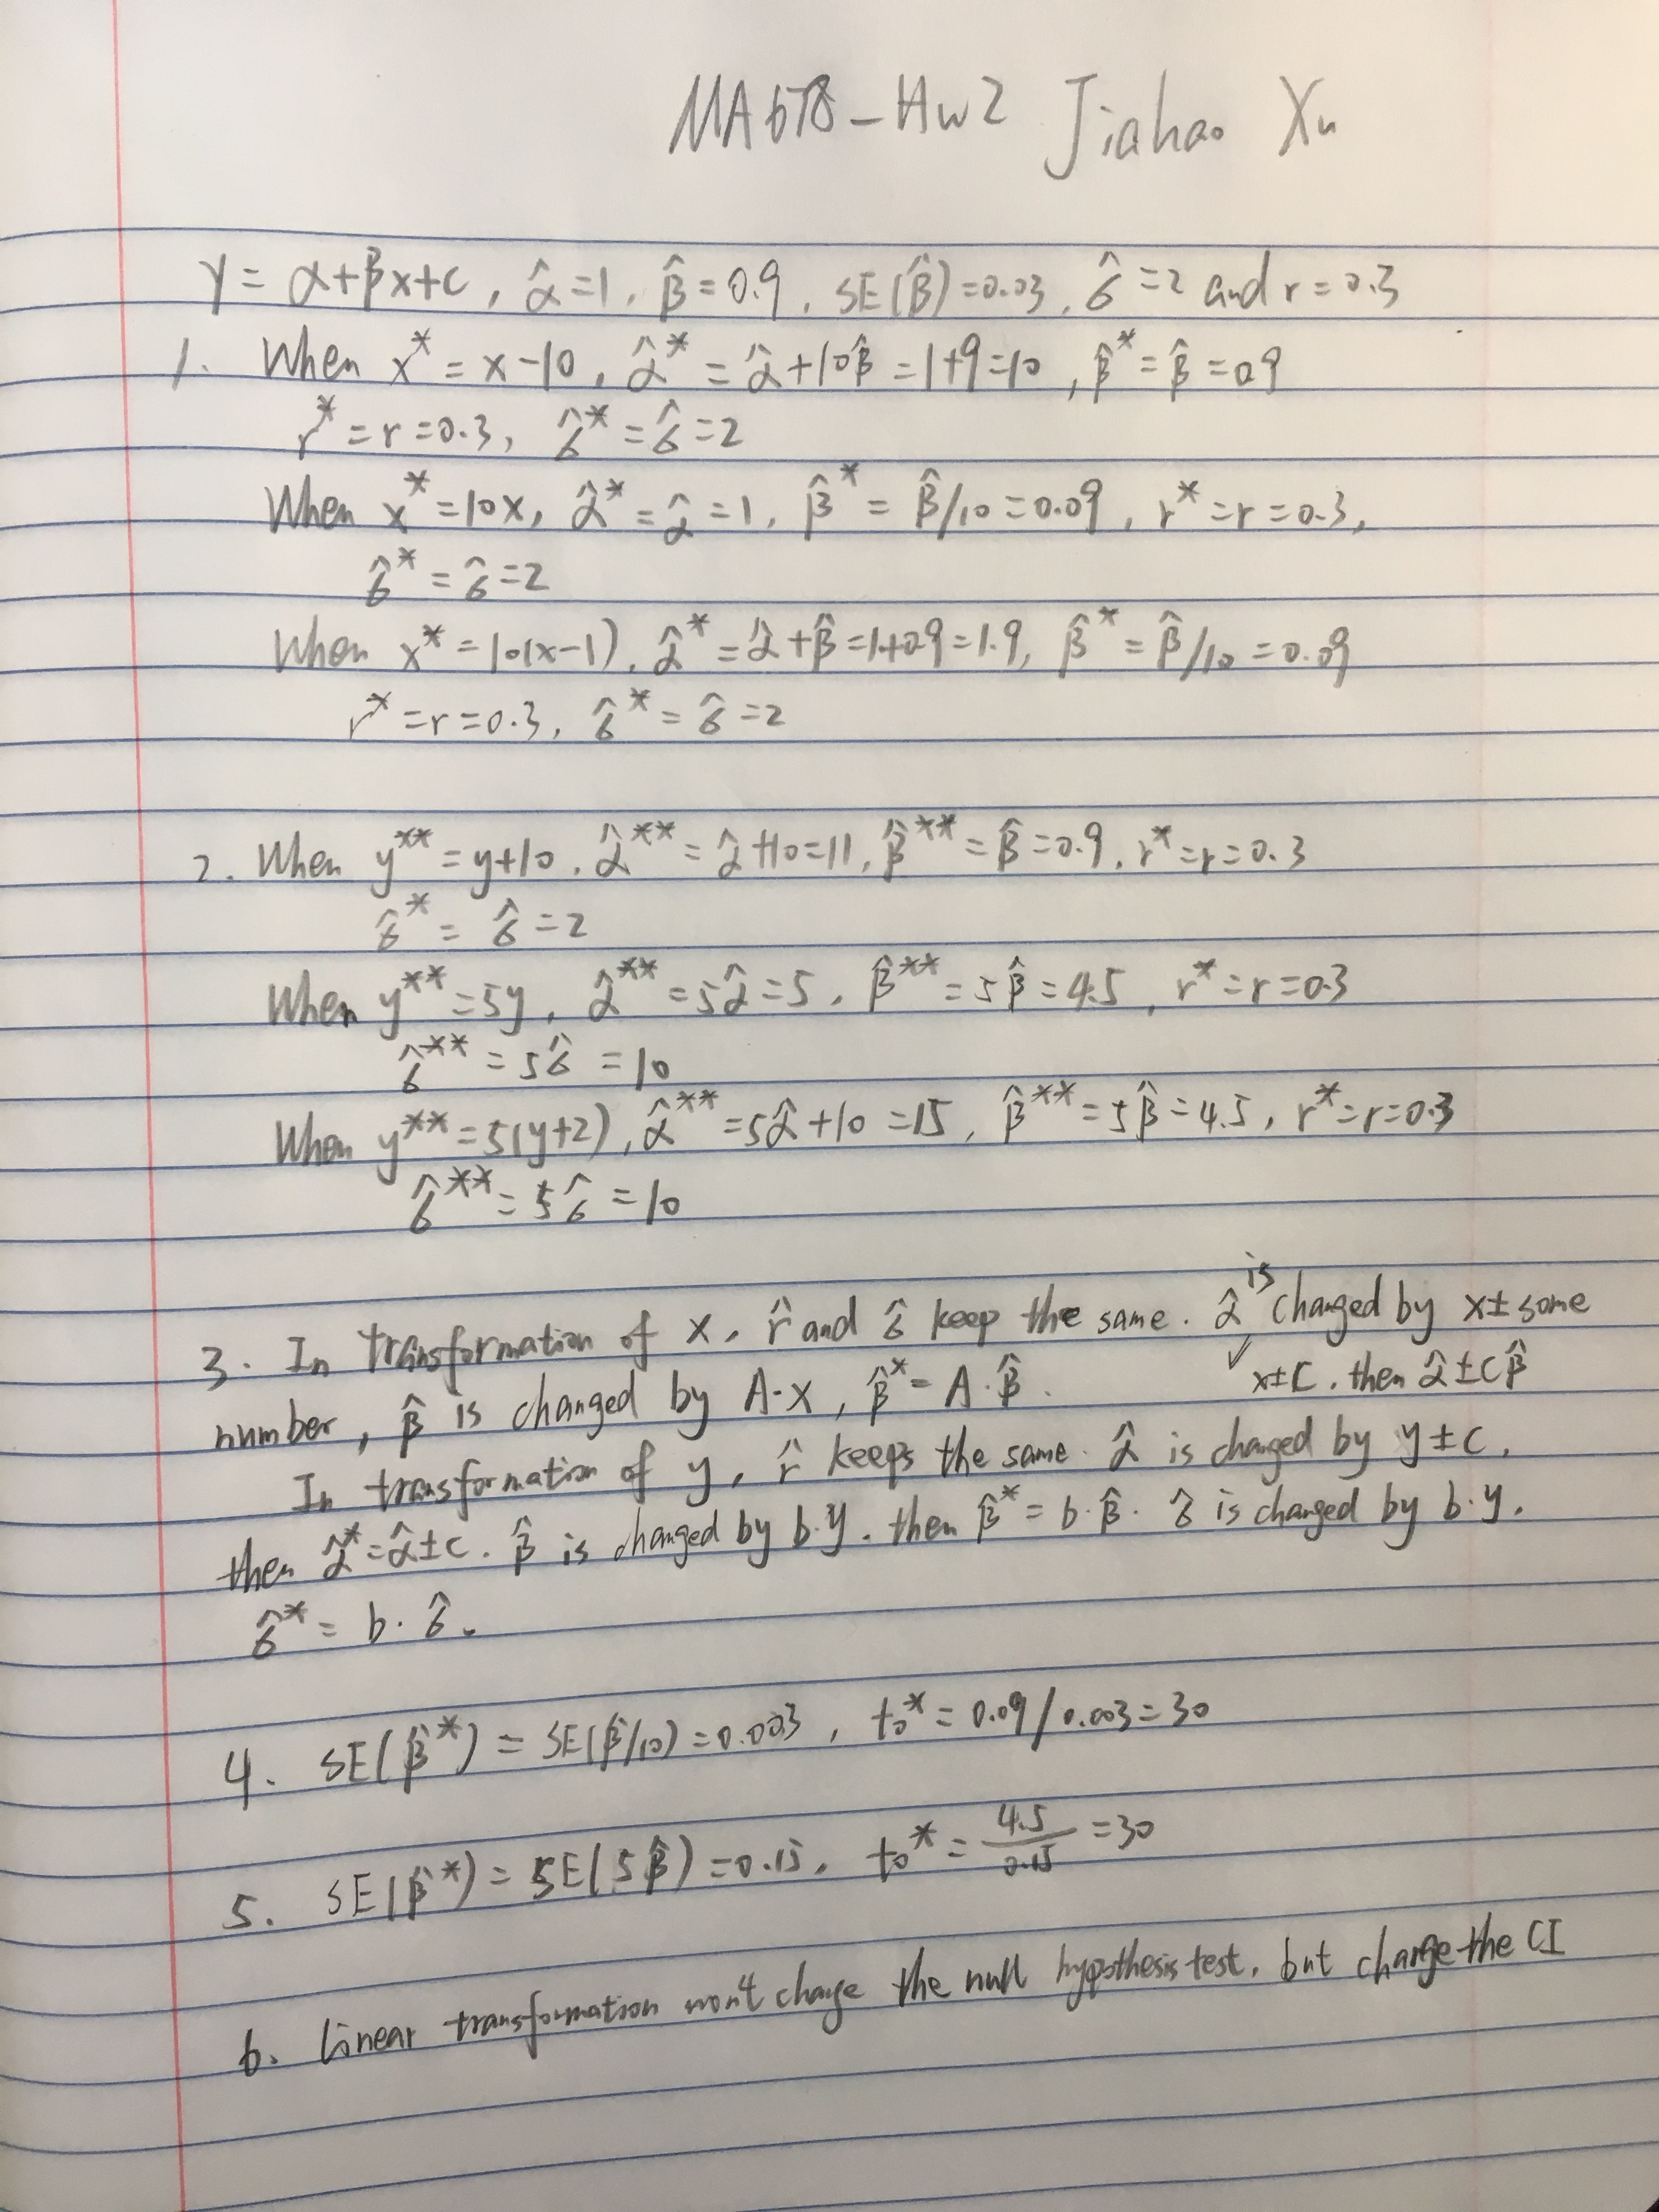
\includegraphics{hw2.jpg}
\caption{Hw2\_byhands part}
\end{figure}

\section{Feedback comments etc.}\label{feedback-comments-etc.}

If you have any comments about the homework, or the class, please write
your feedback here. We love to hear your opinions.


\end{document}
